\section{Multifrequency Analysis}
The Multifrequency Analysis was developed as part of our Beat Detection project to improve the accuracy and reliability of BPM estimation. This analysis technique captures various frequency ranges within an audio signal, enabling a more precise BPM analysis. It is important to note that we are still in the active development phase. For educational purposes and ease of use, we implemented this manually to mimic the functionality of a Discrete Wavelet Transform (DWT). \\

It is also worth noting that this section is a work in progress and will be updated as we continue to develop and refine our Multifrequency Analysis algorithm. The following sections provide an overview of the functionality, algorithm, parameters, and statistical analysis of the Multifrequency Analysis component of our Beat Detection project.

\subsection{Functionality}
The Multifrequency Analysis code is intended to perform a thorough examination of various frequency ranges in an audio signal. This is accomplished by dividing the signal into different frequency bands and analyzing each band separately to extract its BPM. Analyzing different frequency ranges separately allows for the calculation of a mean value, which provides a more accurate indication of the signal's BPM.

\subsection{Algorithm}
This algorithm uses a recursive filtering method to calculate the Beats per Minute (BPM) from an audio signal. First, it checks if the cutoff frequency for the filter exceeds a certain threshold. If the check is positive, the signal is processed with a high-pass filter, and BPM is calculated from it. The results are then stored in an array. Next, the signal is processed with a low-pass filter. The process is recursively repeated for the low-pass filtered signal, with the cutoff frequency halved each time to analyze a broader frequency band. This recursive filtering enables a step-by-step analysis of the signal across different frequency ranges, resulting in more precise BPM values. The final output is an array that contains all the calculated BPM values.

\subsection{Parameters}
\begin{itemize}
    \item \texttt{signal}: The input signal to be analyzed.
    \item \texttt{fs}: The sampling rate of the signal.
    \item \texttt{cutoffFrequency}: The normalized cutoff frequency for the filter.
    \item \texttt{bpmArray}: An array to store the calculated BPM values.
\end{itemize}

\subsection{Statistical Analysis}

The following table presents the results of the BPM analysis using our Multifrequency Analysis algorithm across different music genres and normalized frequency bands. The table includes the actual BPM of the songs, the BPM estimated by our algorithm, and the BPM estimated by an established BPM detection tool (bpm-tools) for comparison.

\begin{table}[H]
    \centering
    \small
    \begin{tabular}{|c|c|c|c|c|c|c|c|c|}
        \hline
        \textbf{Song} & \textbf{Genre} & \textbf{50-100\%} & \textbf{25-50\%} & \textbf{12.5-25\%} & \textbf{0-12.5\%} & \textbf{Our BPM} & \textbf{bpm-tools} & \textbf{Actual} \\ \hline
        1 & Hypertechno & 114.69 & 122.63 & 141.18 & 142.95 & 130.365 & 139.562 & 138 \\ \hline
        2 & Pop Rock & 97.658 & 111.787 & 131.217 & 140.797 & 120.365 & 145.685 & 115 \\ \hline
        3 & Vocal Jazz & 96.721 & 95.074 & 137.276 & 112.713 & 110.4461 & 95.981 & 95 \\ \hline
        4 & Hypertechno & 142.02 & 142.07 & 140.48 & 140.66 & 138.229 & 141.3104 & 142 \\ \hline
        5 & Synthpop & 120.21 & 124.84 & 142.01 & 136.70 & 130.9409 & 118.567 & 118 \\ \hline
    \end{tabular}
    \caption{BPM analysis results across different frequency bands for various music genres}
    \label{tab:bpm_analysis}
\end{table}

The table displays the results of the BPM analysis utilizing our beat detection algorithm across various normalized frequency ranges (0\%-25\%, 12.5\%-25\%, 25\%-50\%, and 50\%-100\%) for different music genres. In general, our algorithm consistently estimates BPM across different frequency bands, with slight variations observed depending on the genre and frequency range. Notably, our algorithm tends to produce BPM estimates that closely align with the actual BPM for genres like Hypertechno and Synthpop, across all frequency bands. However, for Pop Rock and Vocal Jazz, there are instances where the BPM estimates deviate more significantly from the actual BPM, particularly in the higher frequency bands (50\%-100\%). The observation indicates that the algorithm may require further refinement, such as adjusting the weighting or processing of high-frequency components, to enhance accuracy across various music genres. Despite these variations, the algorithm generally demonstrates promising performance in BPM estimation, highlighting its potential usefulness in music analysis applications.

\subsection{Statistical Analysis and Visualization}
In our ongoing development of a beat detection algorithm that utilizes multi-frequency analysis, we have observed some initial trends that warrant discussion regarding our current state of progress. The analysis of normalized autocorrelation functions (ACF) over lag, across different frequency bands (50-100\%, 25-50\%, 12.5-25\%, and 0-12.5\%), has revealed a similarity in the ACF profiles across these spectrums. This similarity indicates a consistent temporal structure of beats, although the highest frequency band (50-100\%) occasionally exhibits a slightly divergent pattern. Therefore, it may be necessary to exclude or differently weight this band in beat detection for specific music genres due to its distinct characteristics and possible introduction of noise, particularly in genres less focused on high-frequency percussive sounds.

\begin{figure}[H]
    \centering
    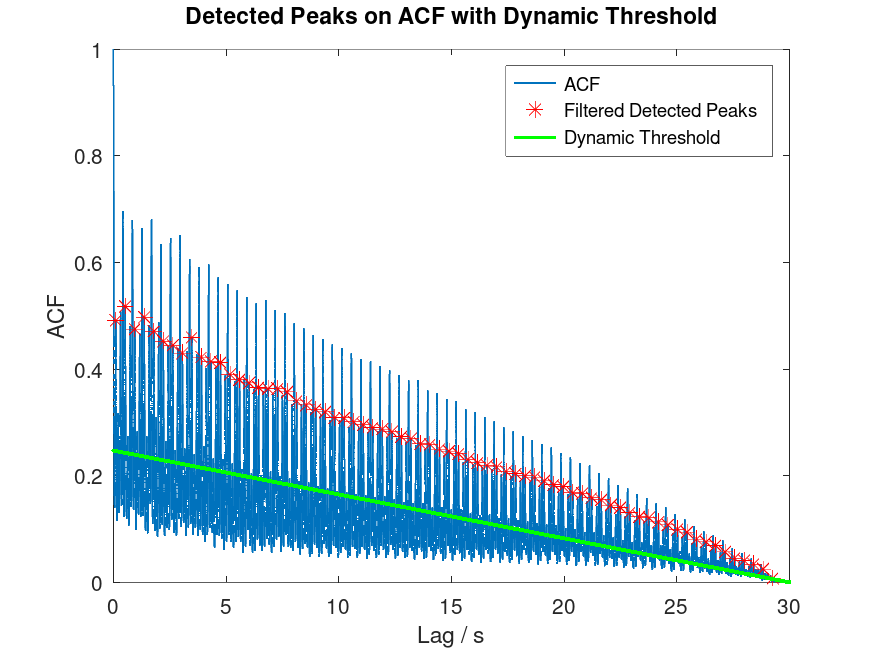
\includegraphics[width=0.8\textwidth]{peaks1.png}
    \caption{Normalized Autocorrelation Function Peaks Across Frequency Bands of Song 4: frequency band 0\%-12.5\%}
\end{figure}

\begin{figure}[H]
    \centering
    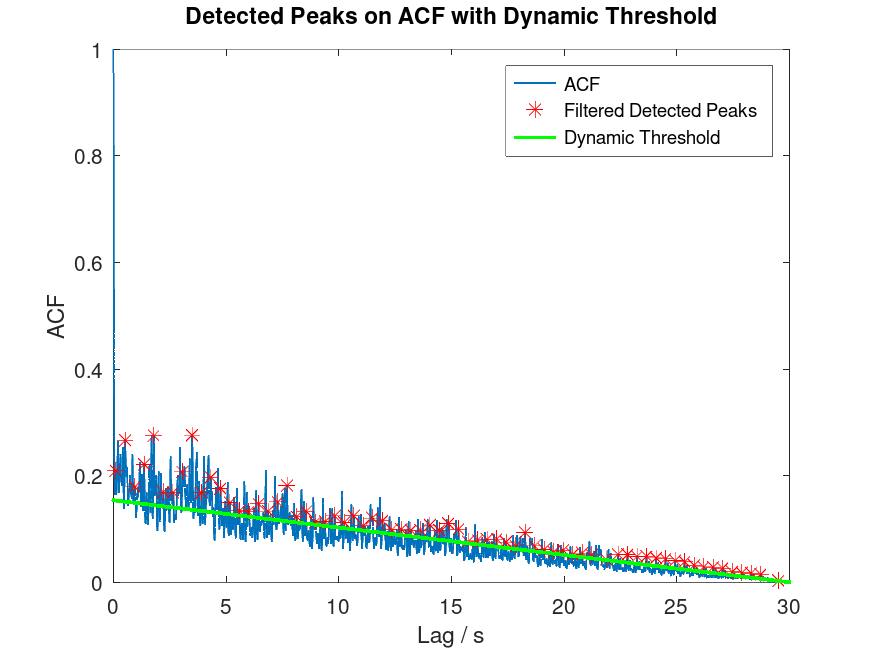
\includegraphics[width=0.8\textwidth]{peaks2.png}
    \caption{Normalized Autocorrelation Function Peaks Across Frequency Bands of Song 4: frequency band 12.5\%-25\%}
\end{figure}

\begin{figure}[H]
    \centering
    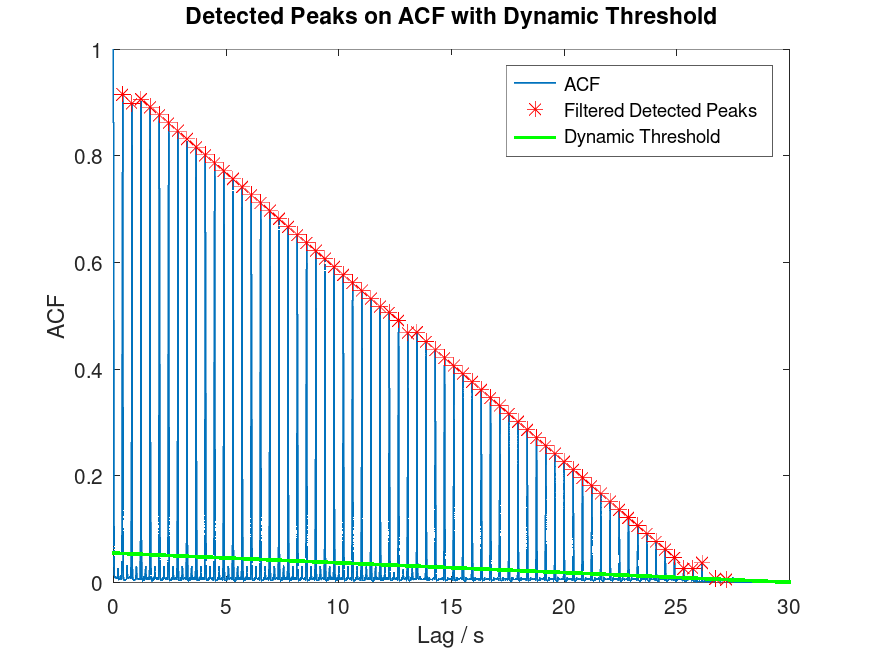
\includegraphics[width=0.8\textwidth]{peaks3.png}
    \caption{Normalized Autocorrelation Function Peaks Across Frequency Bands of Song 4: frequency band 25\%-50\%}
\end{figure}

\begin{figure}[H]
    \centering
    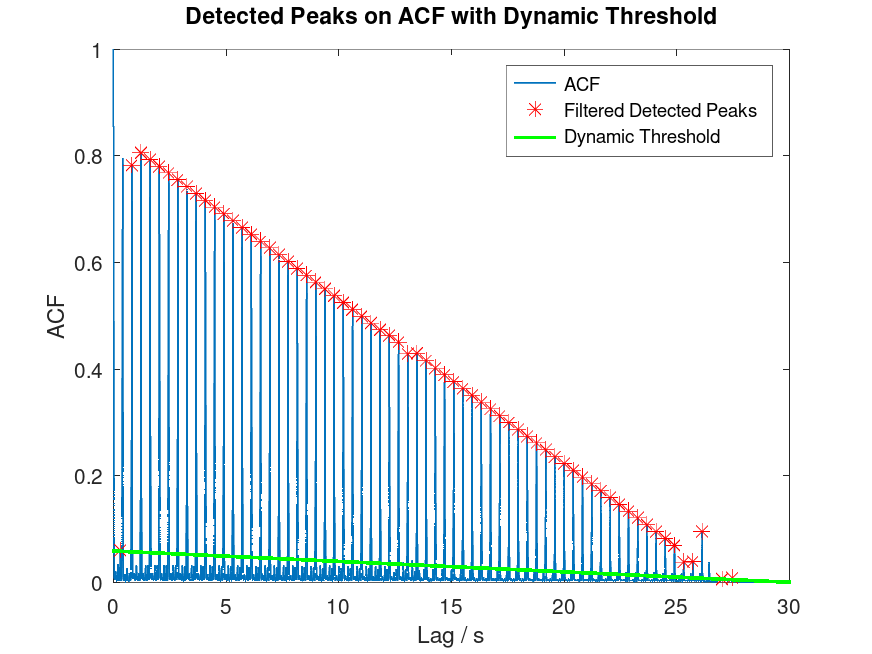
\includegraphics[width=0.8\textwidth]{peaks4.png}
    \caption{Normalized Autocorrelation Function Peaks Across Frequency Bands of Song 4: frequency band 50\%-100\%}
\end{figure}

Currently, our algorithm applies an equal weighting scheme to each detected beat across the frequency bands. However, this method may not be optimal as the significance of beats varies across different frequency ranges. Our preliminary findings regarding the frequency bands' contribution to beat detection highlight the critical and challenging task of parameterization within our algorithm. Our work is currently in the experimental phase. These observations will serve as a basis for further discussion and refinement. The task ahead involves adjusting the weighting of different frequency bands' contributions and possibly reevaluating the inclusion of the highest frequency band for some music genres. This stage of development is critical because it involves carefully considering the spectral content of music and the rhythmic prominence of different frequency ranges to improve the accuracy of our beat detection algorithm. \\

After reevaluating the performance of our beat detection algorithm using the same test protocol on Tidal's Top 100 tracks, our findings indicate that our algorithm has an average BPM detection rate of 124.479, while bpm-tools averages at 121.313 BPM. Additionally, the median BPM detected by our system is 125.5, compared to 122.846 by bpm-tools. The median percent difference between the detected BPM values of the two systems stands at 1.59\%, showcasing a modest improvement in alignment compared to our previous assessments. \\

This improvement highlights the fact that significant advancements in beat detection accuracy are more dependent on fine-tuning algorithmic parameters than on broad-stroke feature development. During this phase of our project, we allocated a considerable amount of development time to refine our multi-frequency analysis approach. In hindsight, we realized that while feature enhancement was critical, parameter optimization is paramount. Moving forward, we must dedicate efforts to meticulously calibrating the algorithm's parameters to yield more significant improvements in performance. Our future development trajectory aims for a balanced approach, pursuing both innovative feature development and rigorous parameter optimization concurrently to achieve optimal beat detection accuracy.

\subsection{Conclusion}
In summary, the Multifrequency Analysis component of our Beat Detection project has shown promising results in enhancing BPM estimation accuracy through the detailed examination of audio signals across various frequency bands. Our recent statistical analysis and performance reevaluation underline the incremental improvements we have achieved, particularly in aligning our BPM detection rates more closely with established tools. However, these findings also highlight the critical role of parameter optimization in achieving significant accuracy gains beyond mere feature enhancement. Our development journey has been a learning curve, emphasizing that beat detection precision is intricately linked to the delicate balance between innovative algorithmic features and meticulous parameter tuning. As we refine our approach, we will increasingly focus on optimizing these parameters to maximize the effectiveness and reliability of our beat detection algorithm. This process is crucial to advancing the state-of-the-art in audio analysis and setting new benchmarks for BPM detection technology.
